\subsection{OVERVIEW}
Given the nature of the application, a three layer approach has been chosen.\newline
\begin{figure}[h!]
	\centering
	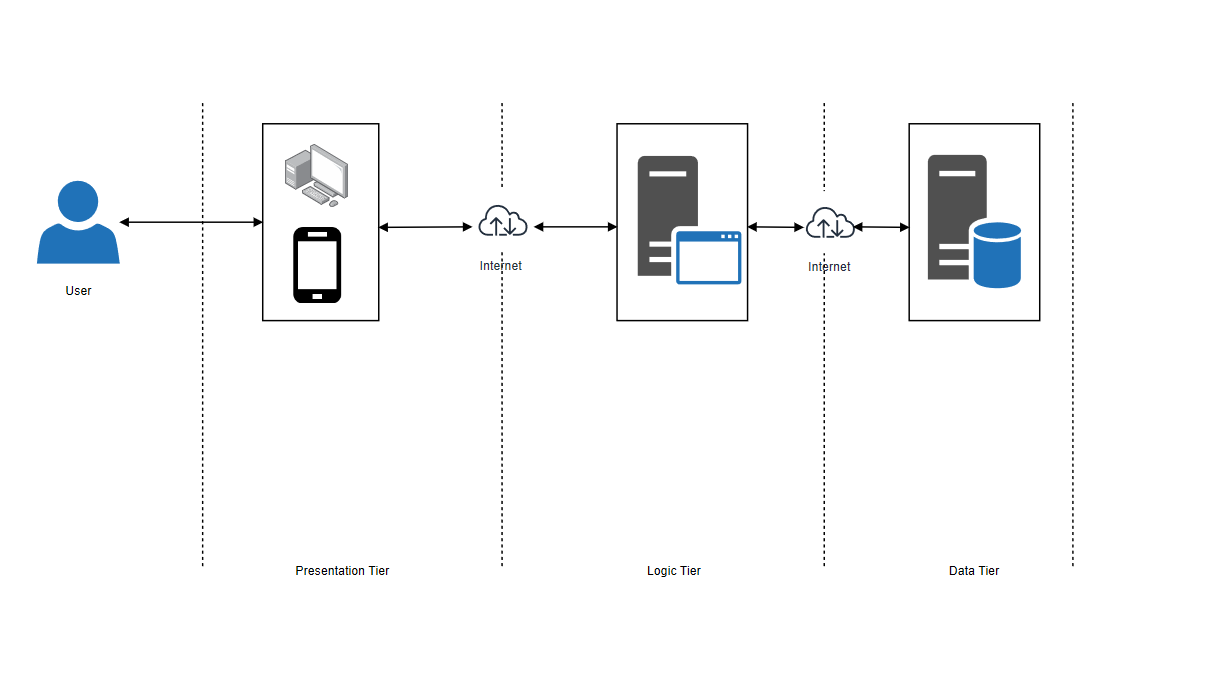
\includegraphics[width=\textwidth]{Images/three_layer}
	\caption{Three layer structure}
\end{figure}
\newline
As shown by the image above, the three layers consist in the presentation tier, the logic tier and the data tier
\begin{itemize}
\item Presentation Tier: consists of the user interfaces for all of the three clients (RegularUser, Policeman and MunicipalAuthority) and is used by the user to interact with both the application logic and Google Mapd APIs \newline
\item Logic Tier: consists of the servers used to control the functionalities of the application, interacts with both the presentation and data tiers \newline
\item Data Tier: consists of the database server (where both user data and data generated by the application are stored), interacts only with the logic tier \newline
\end{itemize}
\newpage
\subsection{COMPONENT VIEW}
\subsubsection{INTRODUCTION}
The following diagram represents the interface structure of the system, focusing on both the application server and the client structure. \newline
\begin{figure}[h!]
	\centering
	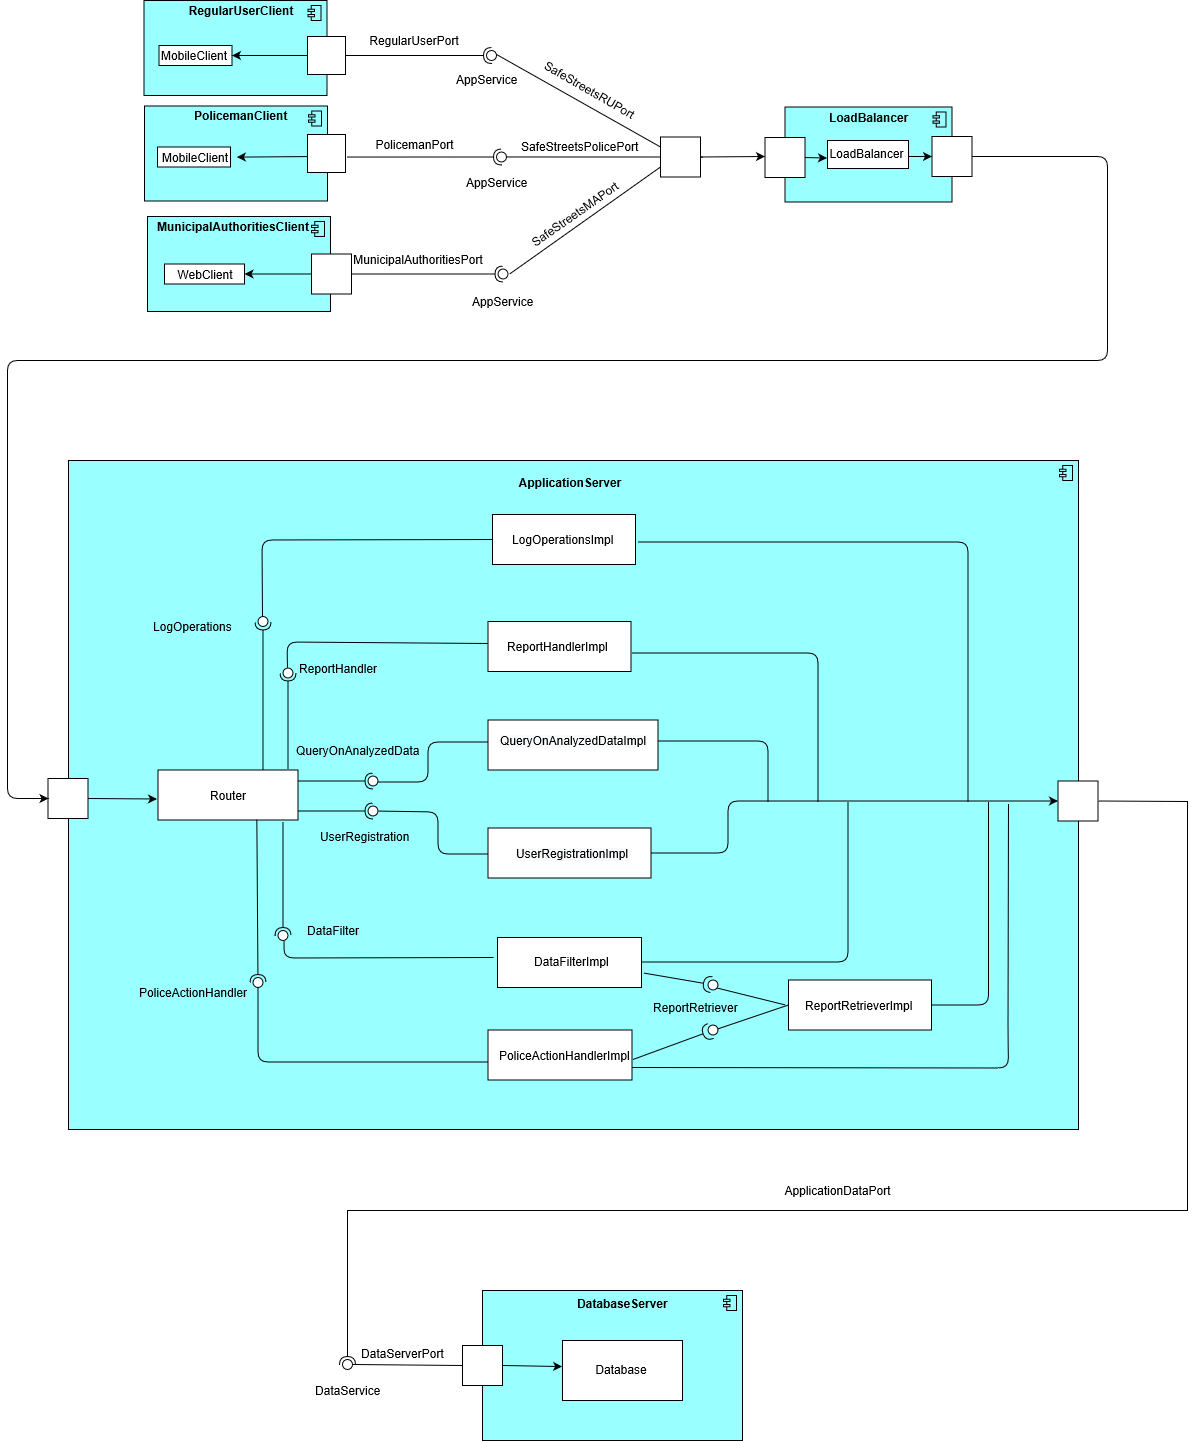
\includegraphics[width=\textwidth]{Images/component_diagram_beta}
	\caption{Schema representing the interfaces}
\end{figure}

As shown above, the greatest part of the application logic is stored on the application server, while the clients just contain what is mandatory in order to contact the application server.
\subsubsection{INTERFACES}
\begin{itemize}
\item QueryOnAnalizedData: allows the users to access data about the reports in a certain area or other information analized by the MunicipalAuthorities
\item PoliceAction: allows the policemen to take action such as noting themself as dispatched or noting a group of reportd as taken care of
\item RetrieveReports: allows the police to retrieve reports submitted by the users
\item SendReports: allows the user to submit reports
\item RegularUserRegistration: allows the registration of new RegularUser profiles
\item LogOperations: allows all kinds of users to login and logout of the application
\item QueryOnData: allows MunicipalAuthority profiles to make queries on the collected data
\end{itemize}
The logic of the application works based on the afromentioned interfaces: they grant all the functionality needed to satisfy the system's goals.
In the next two pictures more information about the system will be provided via a more accurate version of the class diagram presented in the RASD and a schema about the relationship between the classes interfaces and implementations of said interfaces
\newpage
\begin{figure}[h!]
	\centering
	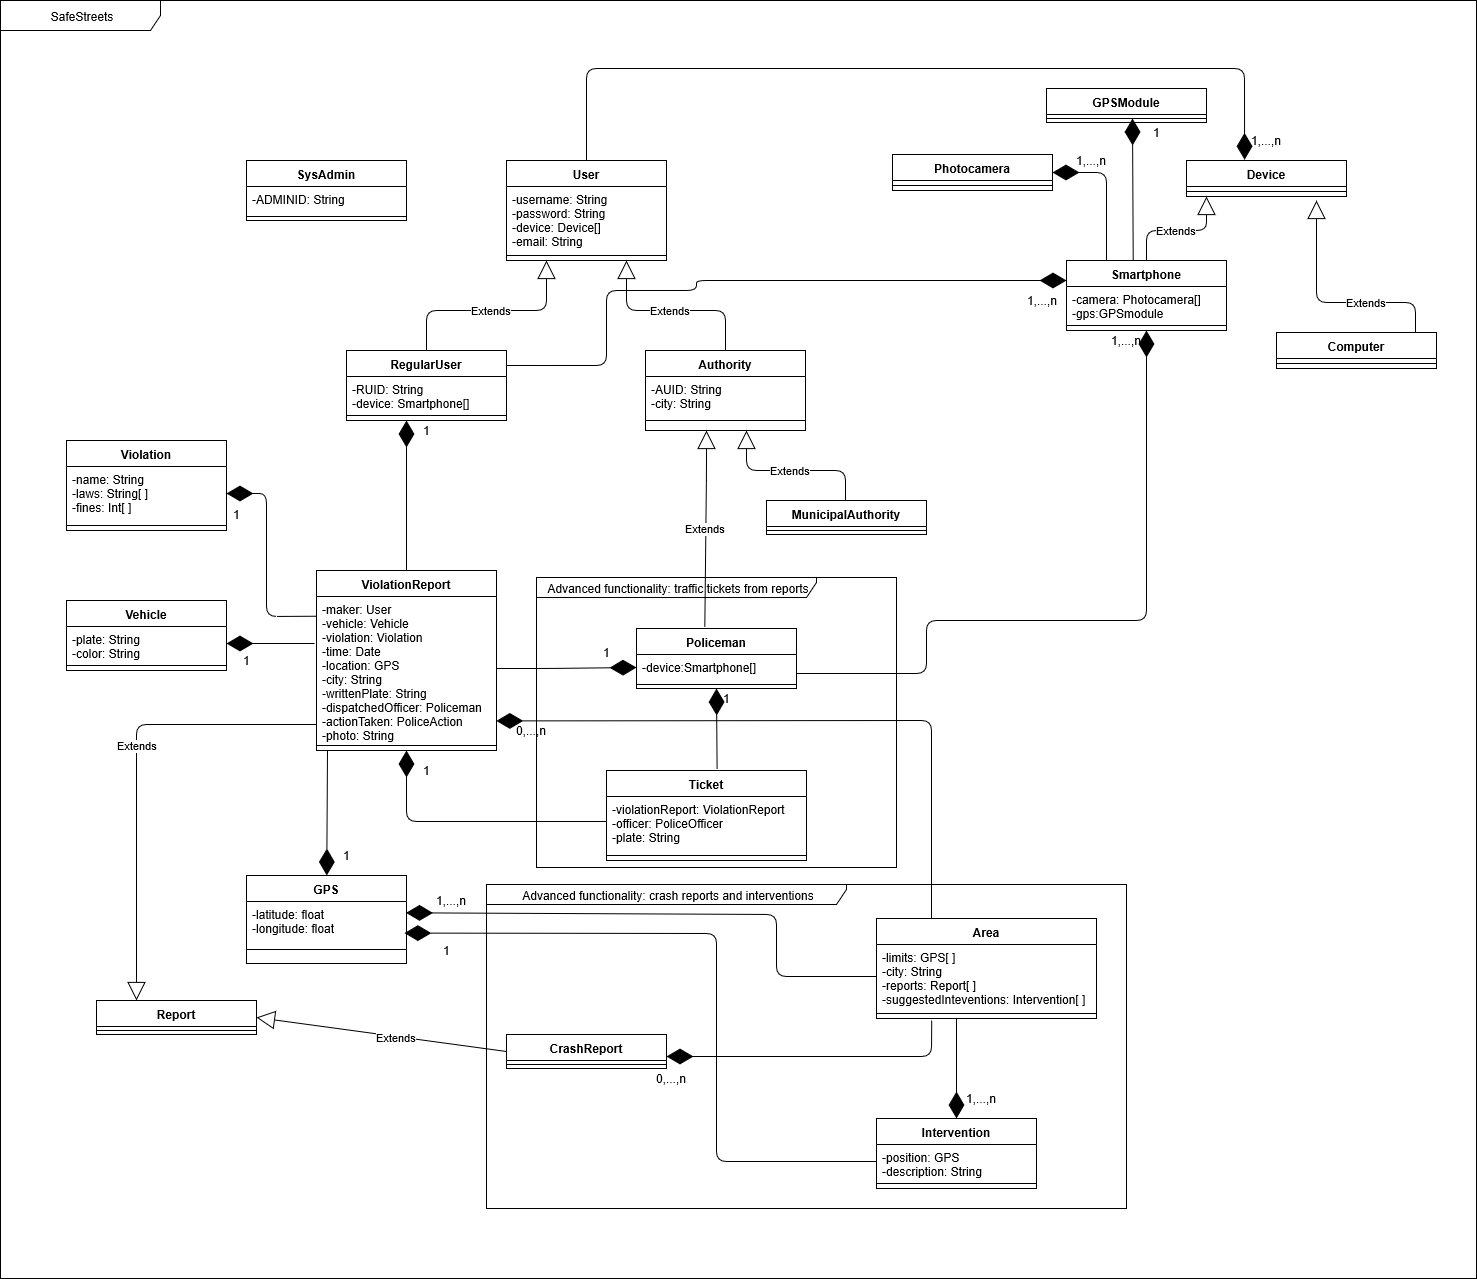
\includegraphics[angle=90, scale=0.45]{Images/ADV_class_diagram}
	\caption{Class diagram}
\end{figure}
\newpage

\begin{figure}[h!]
	\centering
	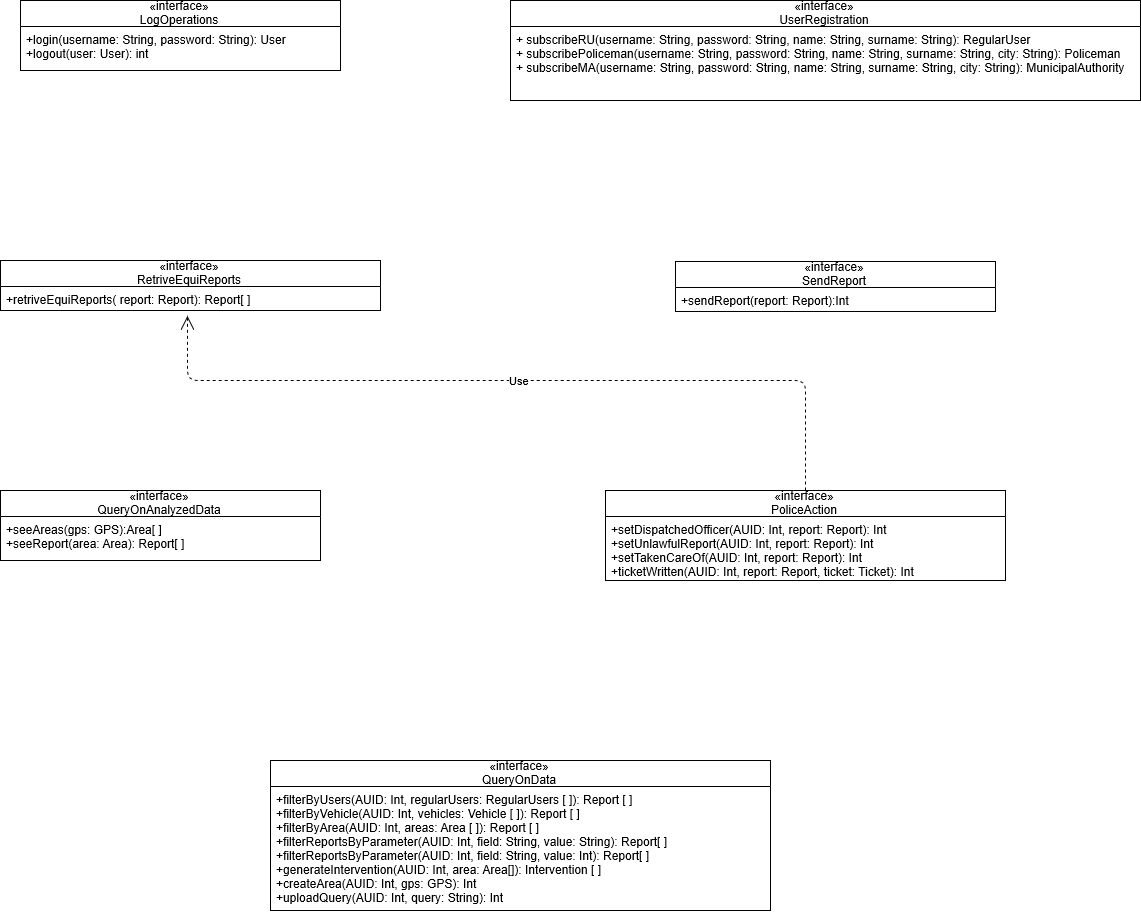
\includegraphics[angle=90, scale=0.28]{Images/interface_diagram}
	\caption{Relation between interfaces and already specified classes}
\end{figure}
\newpage
\subsubsection{DEPLOYMENT VIEW}

\begin{figure}[h!]
	\centering
	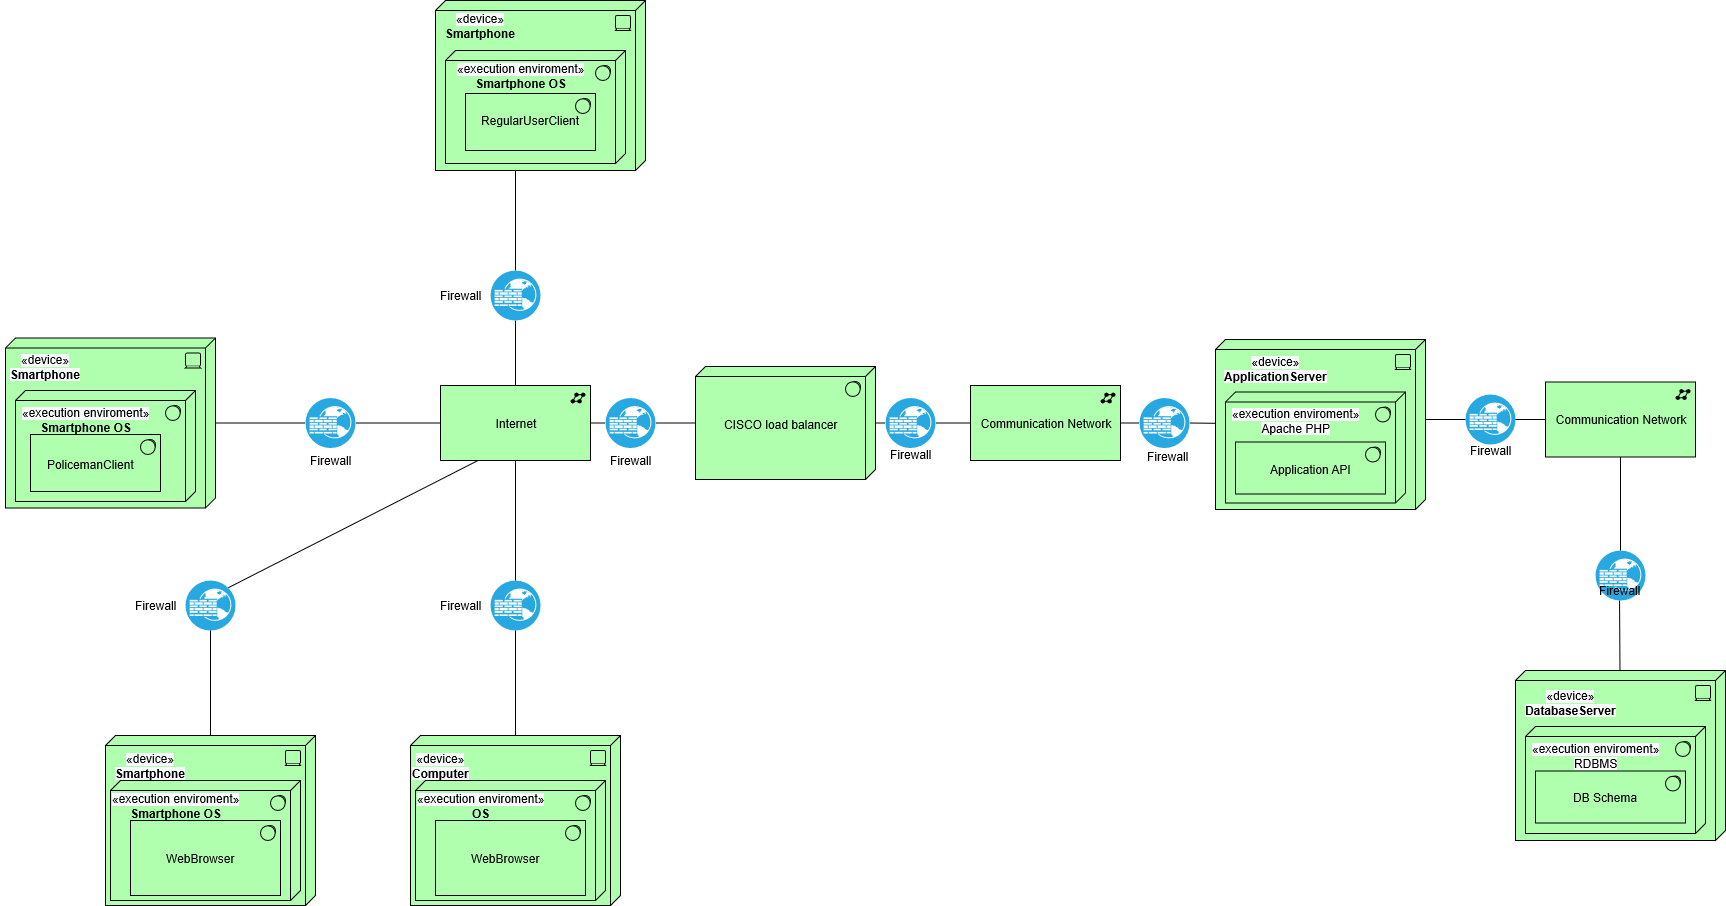
\includegraphics[width=\textwidth]{Images/physical_view}
	\caption{Physical view}
\end{figure}

The image above shows the system's architecture from a phisical standpoint.
Components:
\begin{itemize}
\item Smartphone: Device used by both RegularUser and Policeman users type to interact with the application. Two different clients will be developed: one for regular users, that will allow them to look at already analyzed data and submit reports, and a different one for policemen, that will allow the officers make reports (upon which they will take actions right away) and take actions on reports
\item Computer: device used by MunicipalAuthorities users. They will interact with the application via a web page, that will allow them to interact in various ways with the Reports submitted by the other users.
\item Application server: this server contains the application logic and will interact with the different clients in a client-server way.
\item DatabaseServer: this server contains the actual data, both about the registered users and related to the user submitted reports, the actions taken by the police and the results of the data mining operations done by municipal authorities
\end{itemize}

